%************************************************
\chapter{Introduction}\label{ch:introduction}
%************************************************

Here comes the introduction with a cite \cite{renz2016lak} and a ref \autoref{ch:conclusion} and an acronym \ac{API}.

\begin{figure}[!h]
	\centering
	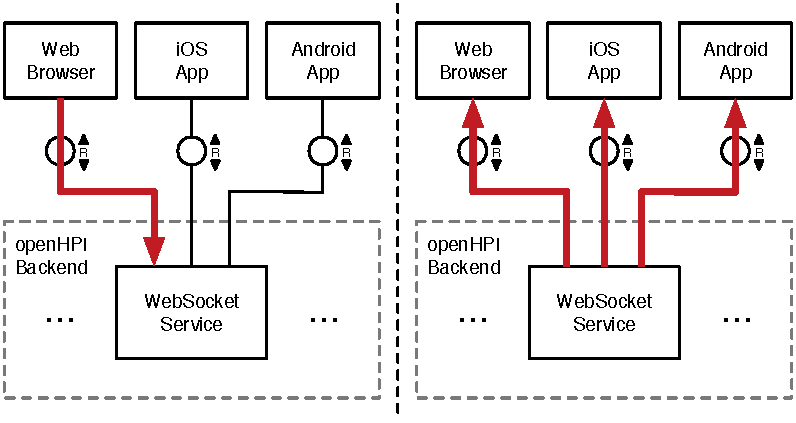
\includegraphics[width=0.8\textwidth]{figures/websocket}
	\caption[A Figure Short-Title]{A Figure Title}
	\label{fig:websocket}
\end{figure}

\section{Motivation}

\begin{table}[!h]
\centering
\begin{tabular}{@{}lllll@{}}
\toprule
Algorithm & Class & Precision & Recall & F-Measure \\ \midrule
SVM       & CoP   & 0.309     & 0.486  & 0.378     \\ \cmidrule(l){2-5} 
          & RoA   & 0.571     & 0.560  & 0.565     \\ \midrule
kNN       & CoP   & 0.391     & 0.344  & 0.366     \\ \cmidrule(l){2-5} 
          & RoA   & 0.623     & 0.660  & 0.641     \\ \midrule
RForest   & CoP   & 0.493     & 0.262  & 0.342     \\ \cmidrule(l){2-5} 
          & RoA   & 0.639     & 0.851  & 0.730     \\ \bottomrule
\end{tabular}
\caption{My First Table}
\label{tab:first-table}
\end{table}

